\documentclass[20pt,a1paper,landscape]{tikzposter}

% required packages
\usepackage{amsmath}
\usepackage{amsfonts}
\usepackage{graphicx}

%% Available themes: see also
%% https://bitbucket.org/surmann/tikzposter/downloads/themes.pdf
\usetheme{Default}
\colorlet{backgroundcolor}{white}

% title information
\title{A Flexible Approach for Predictive Biomarker Discovery}
\author{Philippe Boileau$^1$, Nina Ting Qi$^2$, Mark J. van der Laan$^1$
  Sandrine Dudoit$^1$, Ning Leng$^2$}
\institute{$^1$University of California, Berkeley; $^2$Genentech Inc.}

% dictate default block options
\newcommand{\myblock}[2]{\block[titleinnersep=4mm, linewidth=1mm]{#1}{#2}}
\newcommand{\mysmallblock}[2]{\block[titleinnersep=1mm, linewidth=1mm]{{\small #1}}{{\small#2\par}}}

\begin{document}

% title and graphics
\maketitle[width=23in]
\node[anchor=west] at (TP@title.west) {
\includegraphics[width=8cm]{logos/cal}};
\node[anchor=east] at (TP@title.east) {
\includegraphics[width=7cm]{logos/arxiv-link-qr-code}};

\begin{columns}

  \column{0.333}

  \myblock{Background}{
    \begin{itemize}
      \item Predictive biomarkers are treatment effect modifiers.
      \item In high dimensions, these biomarkers are discovered using
        interpretable conditional average treatment effect estimators, like the
        modified covariates procedures of Tian et al. (2014).
      \item These methods make simplifying assumptions about the
        data-generating process, resulting in a lack of Type-I error rate
        control.
      \item High false discovery rates lead to wasted resources, negatively
        affecting patient outcomes.
    \end{itemize}
  }

  \myblock{Variable Importance Parameter}{
    Consider $n$ identically and independently distributed (i.i.d) full-data
    random vectors $X = (W, A, Y^{(0)}, Y^{(1)}) \sim P_X$.

    \begin{itemize}
      \item $W$: A $p$-length random vector of centered pretreatment biomarkers
        with nonzero variance.
      \item $A$: A random binary indicator of treatment assignment.
      \item $Y^{(0)}, Y^{(1)}$: Continuous potential outcomes under assignment
        to the control and treatment allocations, respectively.
    \end{itemize}

    Our causal variable importance parameter is
    $\Psi^F(P_X) = (\Psi_1^F(P_X), \ldots, \Psi_p^F(P_X))$, where
    \begin{equation*}
      \Psi_j^F(P_X) \equiv \frac{
        \mathbb{E}_{P_X}\left[\left(Y^{(1)}-Y^{(0)}\right)W_j\right]
        }{\mathbb{E}_{P_X}\left[W_j^2\right]}.
    \end{equation*}

    Given access instead to $n$ i.i.d. censored random observations $O = (W, A,
    Y)$ where $Y = AY^{(1)} + (1-A)Y^{(0)}$, $\Psi^F(P_X)$ is identified under
    the assumptions of unmeasured confounding and positivity by $\Psi(P_0) =
    (\Psi_1(P_0), \ldots, \Psi_p(P_0))$. Here,
    \begin{equation*}
      \Psi_j(P_0) \equiv \frac{
        \mathbb{E}_{P_0}\left[\left(\bar{Q}_0(A=1,W)-
        \bar{Q}_0(A=0,W)\right)W_j\right]
        }{\mathbb{E}_{P_0}\left[W_j^2\right]},
    \end{equation*}
    where $\bar{Q}_0(A,W) = \mathbb{E}_{P_0}[Y|A,W]$.
  }

  \column{0.334}
  
  \myblock{Application to IMmotion 150 and 151}{
    \vspace{-1.5em}
    \centering
    \begin{tikzfigure}
      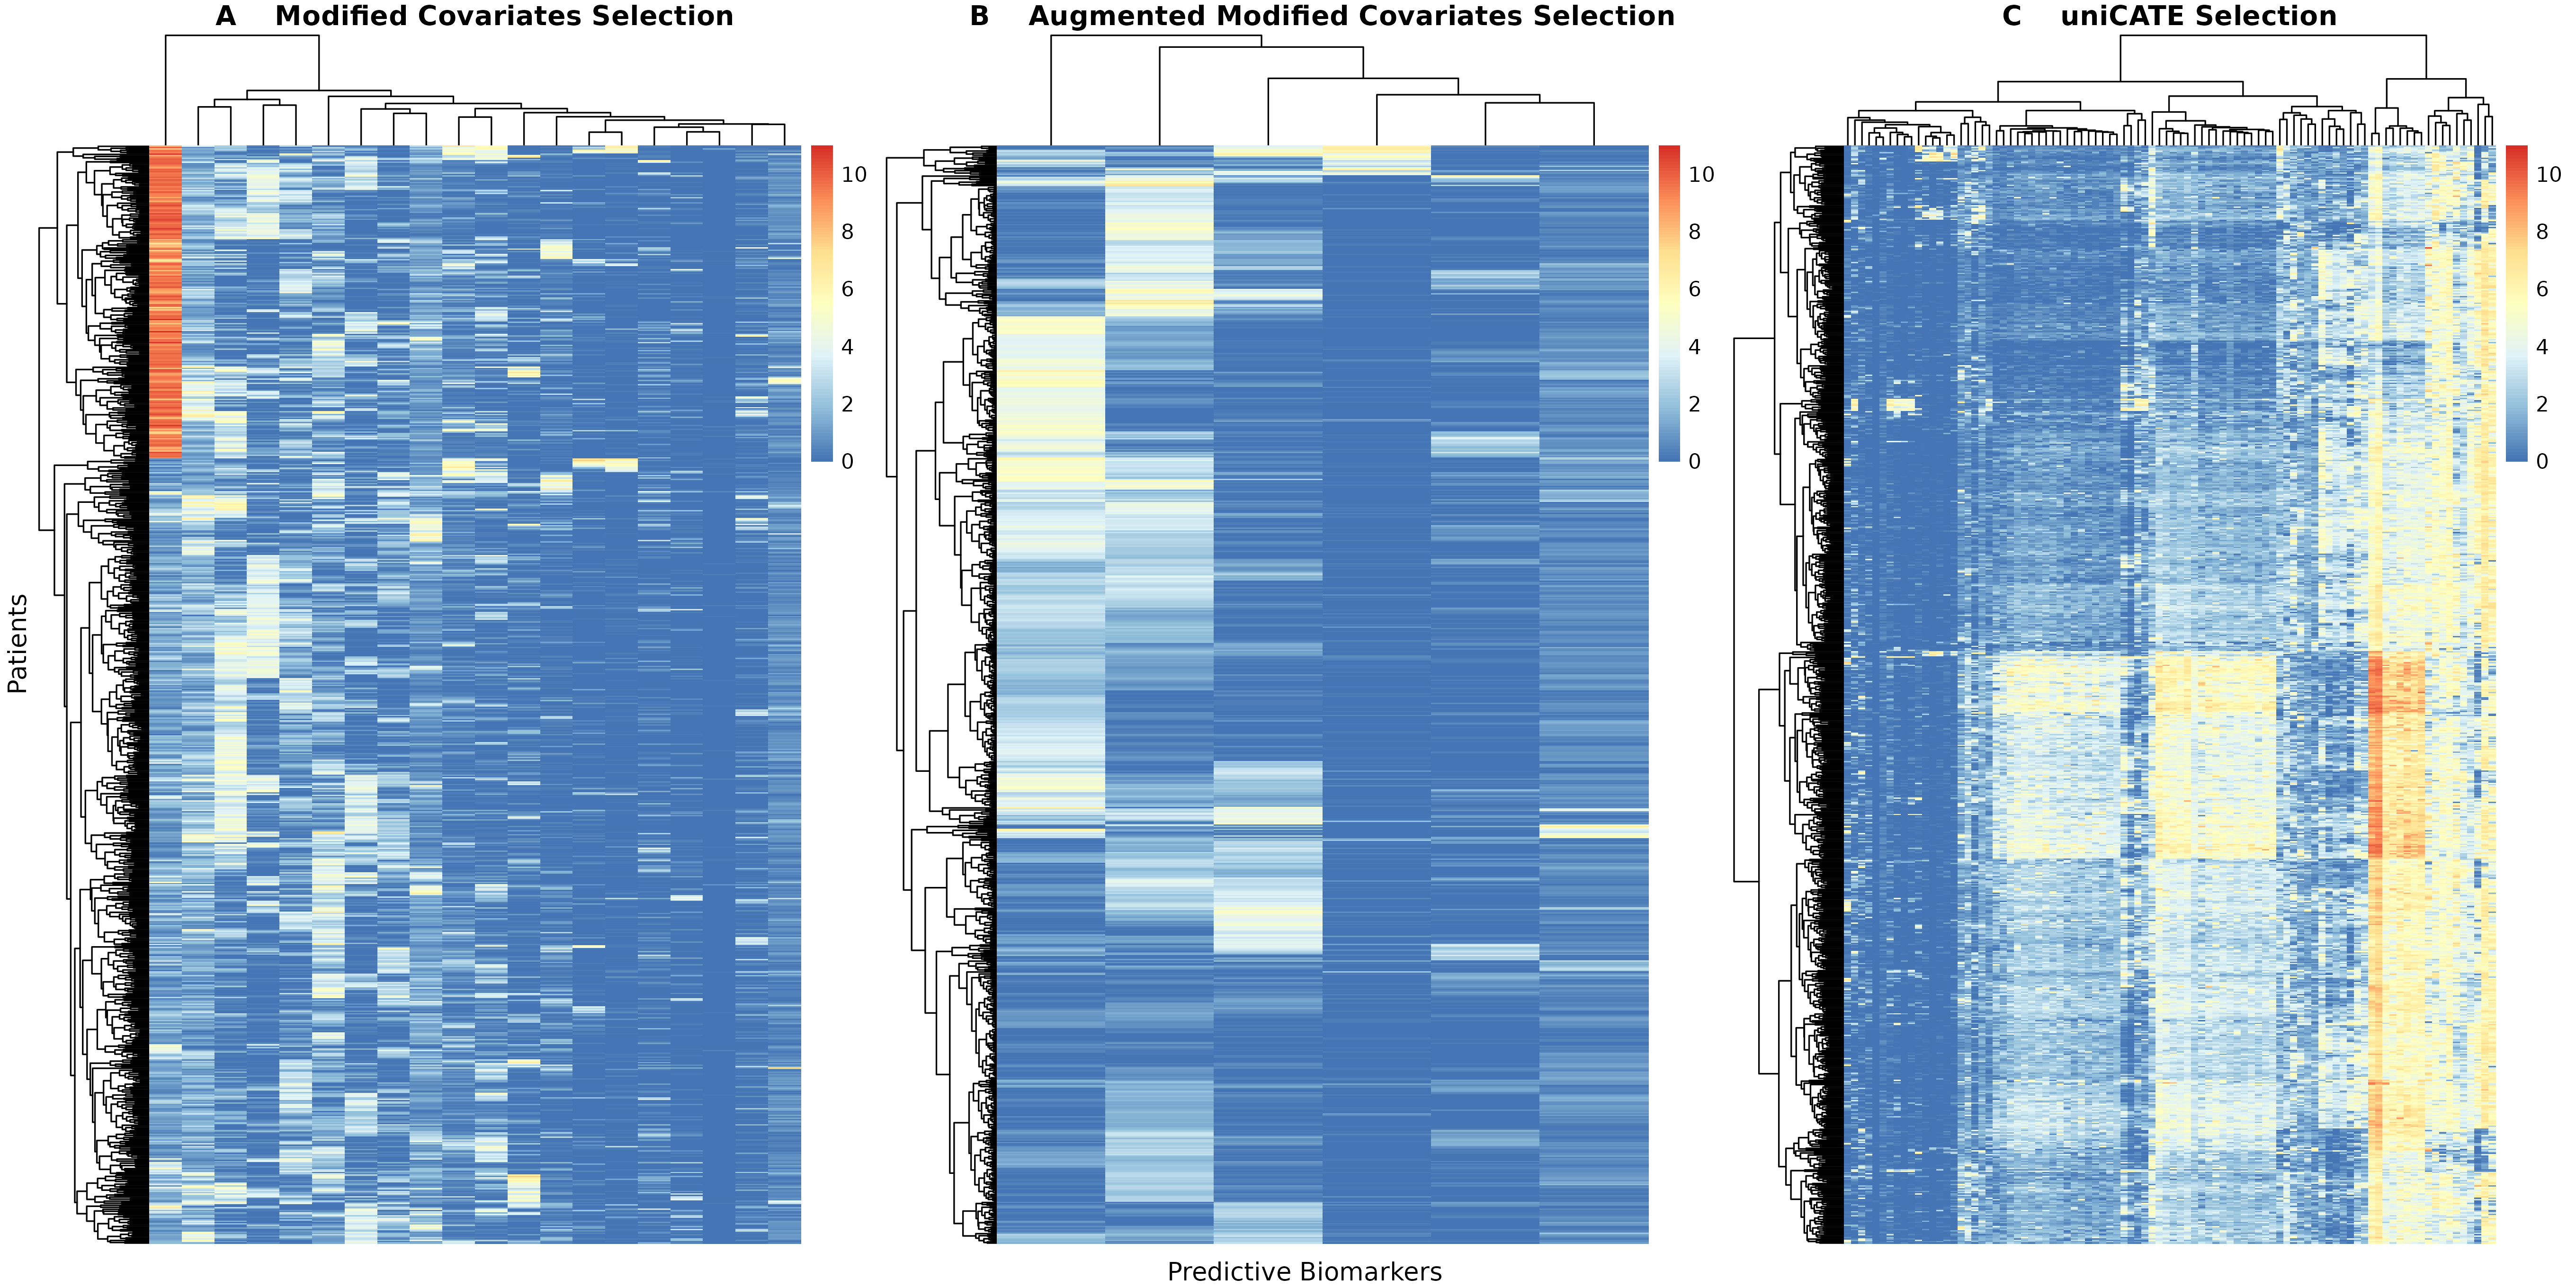
\includegraphics[width=0.295\textwidth]{graphs/heatmaps.png}
    \end{tikzfigure}
    \vspace{-1.5em}
  }
  
  \myblock{Inference}{
    Let $g_0(W) = \mathbb{P}_{P_0}[A=1|W]$, and let $\hat{g}$ and
    $\hat{\bar{Q}}$ be estimators of $g_0$ and $\bar{Q}_0$, respectively.
    Define the Augmented Inverse Probability Weighted outcome difference as
    \begin{align*}
      T(O)
      & \equiv \left(\frac{I(A=1)}{\hat{g}(W)}
        - \frac{I(A=0)}{1 - \hat{g}(W)}\right)
        \left(Y-\hat{\bar{Q}}(A,W)\right) \\
      & \qquad + \hat{\bar{Q}}(1,W)-\hat{\bar{Q}}(0, W).
    \end{align*}

    We derive from the efficient influence function of $\Psi_j(P_0)$, $D_j(O)$,
    the double-robust one-step estimator
    \begin{equation*}
      \hat{\Psi}_j(P_n) \equiv \frac{\sum_{i=1}^n T(O_i) W_{ij}}
      {\sum_{i=1}^n W_{ij}^2},
    \end{equation*}
    where $\sum_i W_{ij} = 0$ for all $j$ and $P_n$ is the empirical
    distribution.

    If $\hat{g}$ and $\hat{\bar{Q}}$ are trained using sample splitting
    techniques, and we assume that $\lVert \hat{g} - g_0 \rVert_2 \lVert
    \hat{\bar{Q}} - \bar{Q}_0\rVert_2 = o_p(n^{-1/2})$, then
    \begin{equation*}
      \sqrt{n}\left(\hat{\Psi}_j(P_n) - \Psi_j(P_0)\right)
      \overset{D}{\rightarrow} N\left(0,
      \mathbb{V}_{P_0}\left[D_j(O)\right]\right).
    \end{equation*}

    \vspace{-1em}
  }

  \mysmallblock{Funding}{
    \vspace{-1em}
    PB gratefully acknowledges the support of the National Science and
    Engineering Research Council of Canada and the Fonds de recherche du
    Qu\'{e}bec -- Nature et technologies.
    \vspace{-1em}
  }
  
  \column{0.333}

  \myblock{Randomized Control Trial Simulations}{
    \vspace{-1.5em}
    \begin{tikzfigure}
      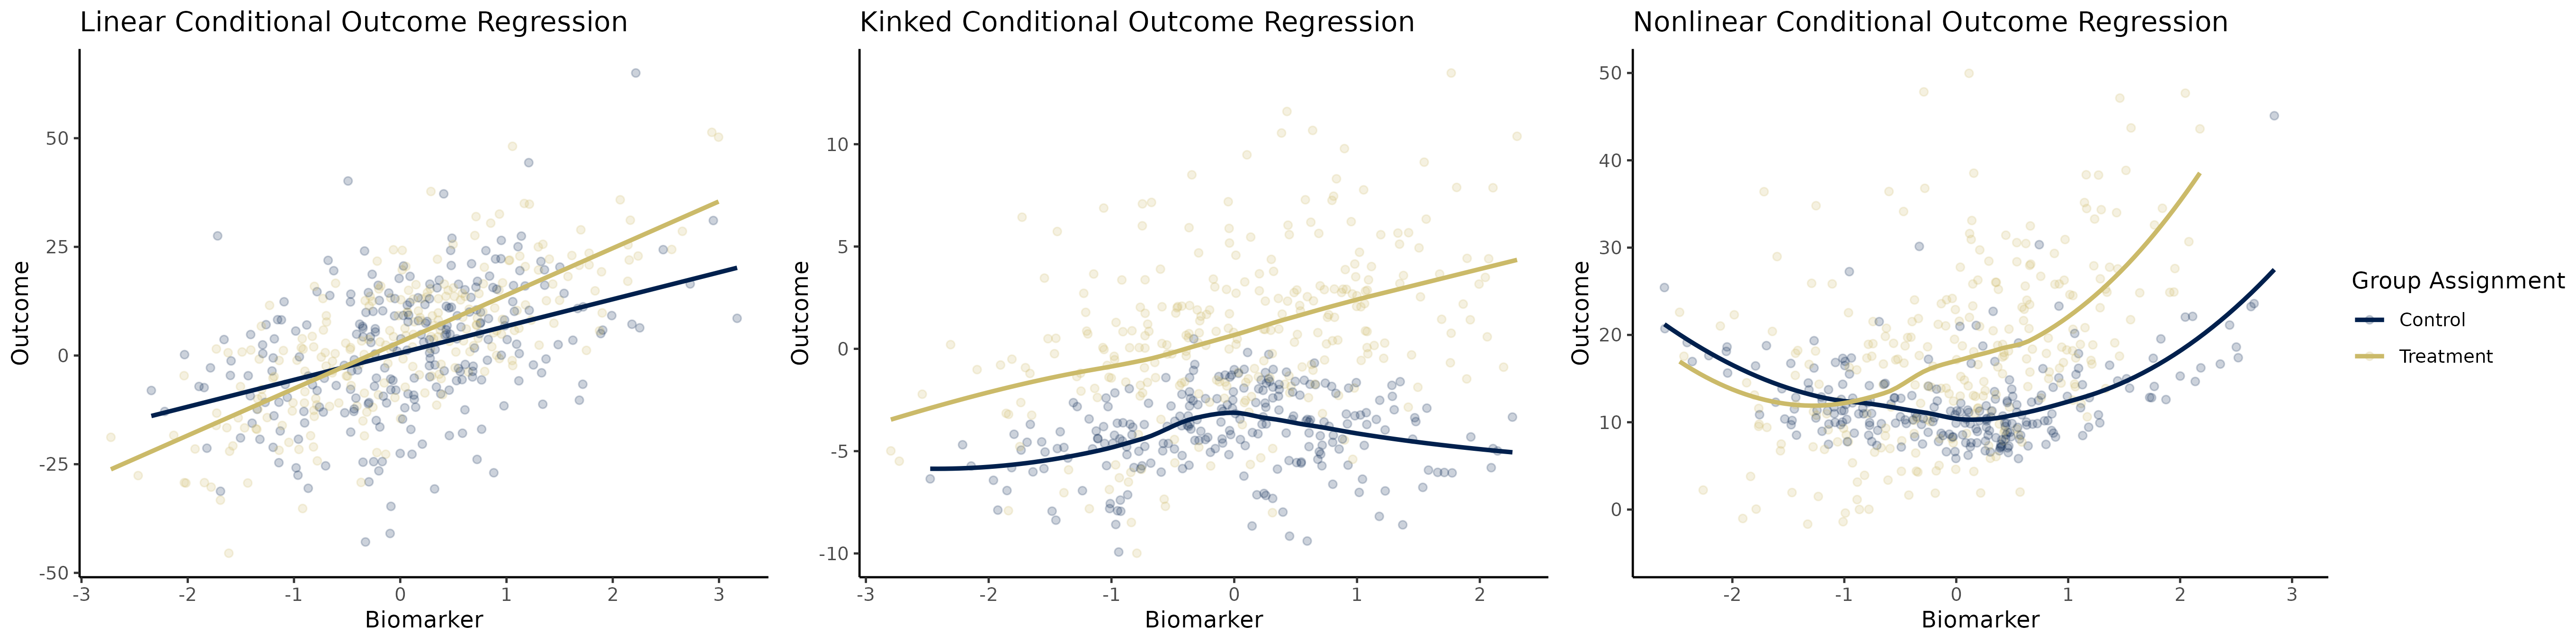
\includegraphics[width=0.29\textwidth]{graphs/dgp-sketches.png}
    \end{tikzfigure}
    \vspace{-3.5em}
    \begin{tikzfigure}
      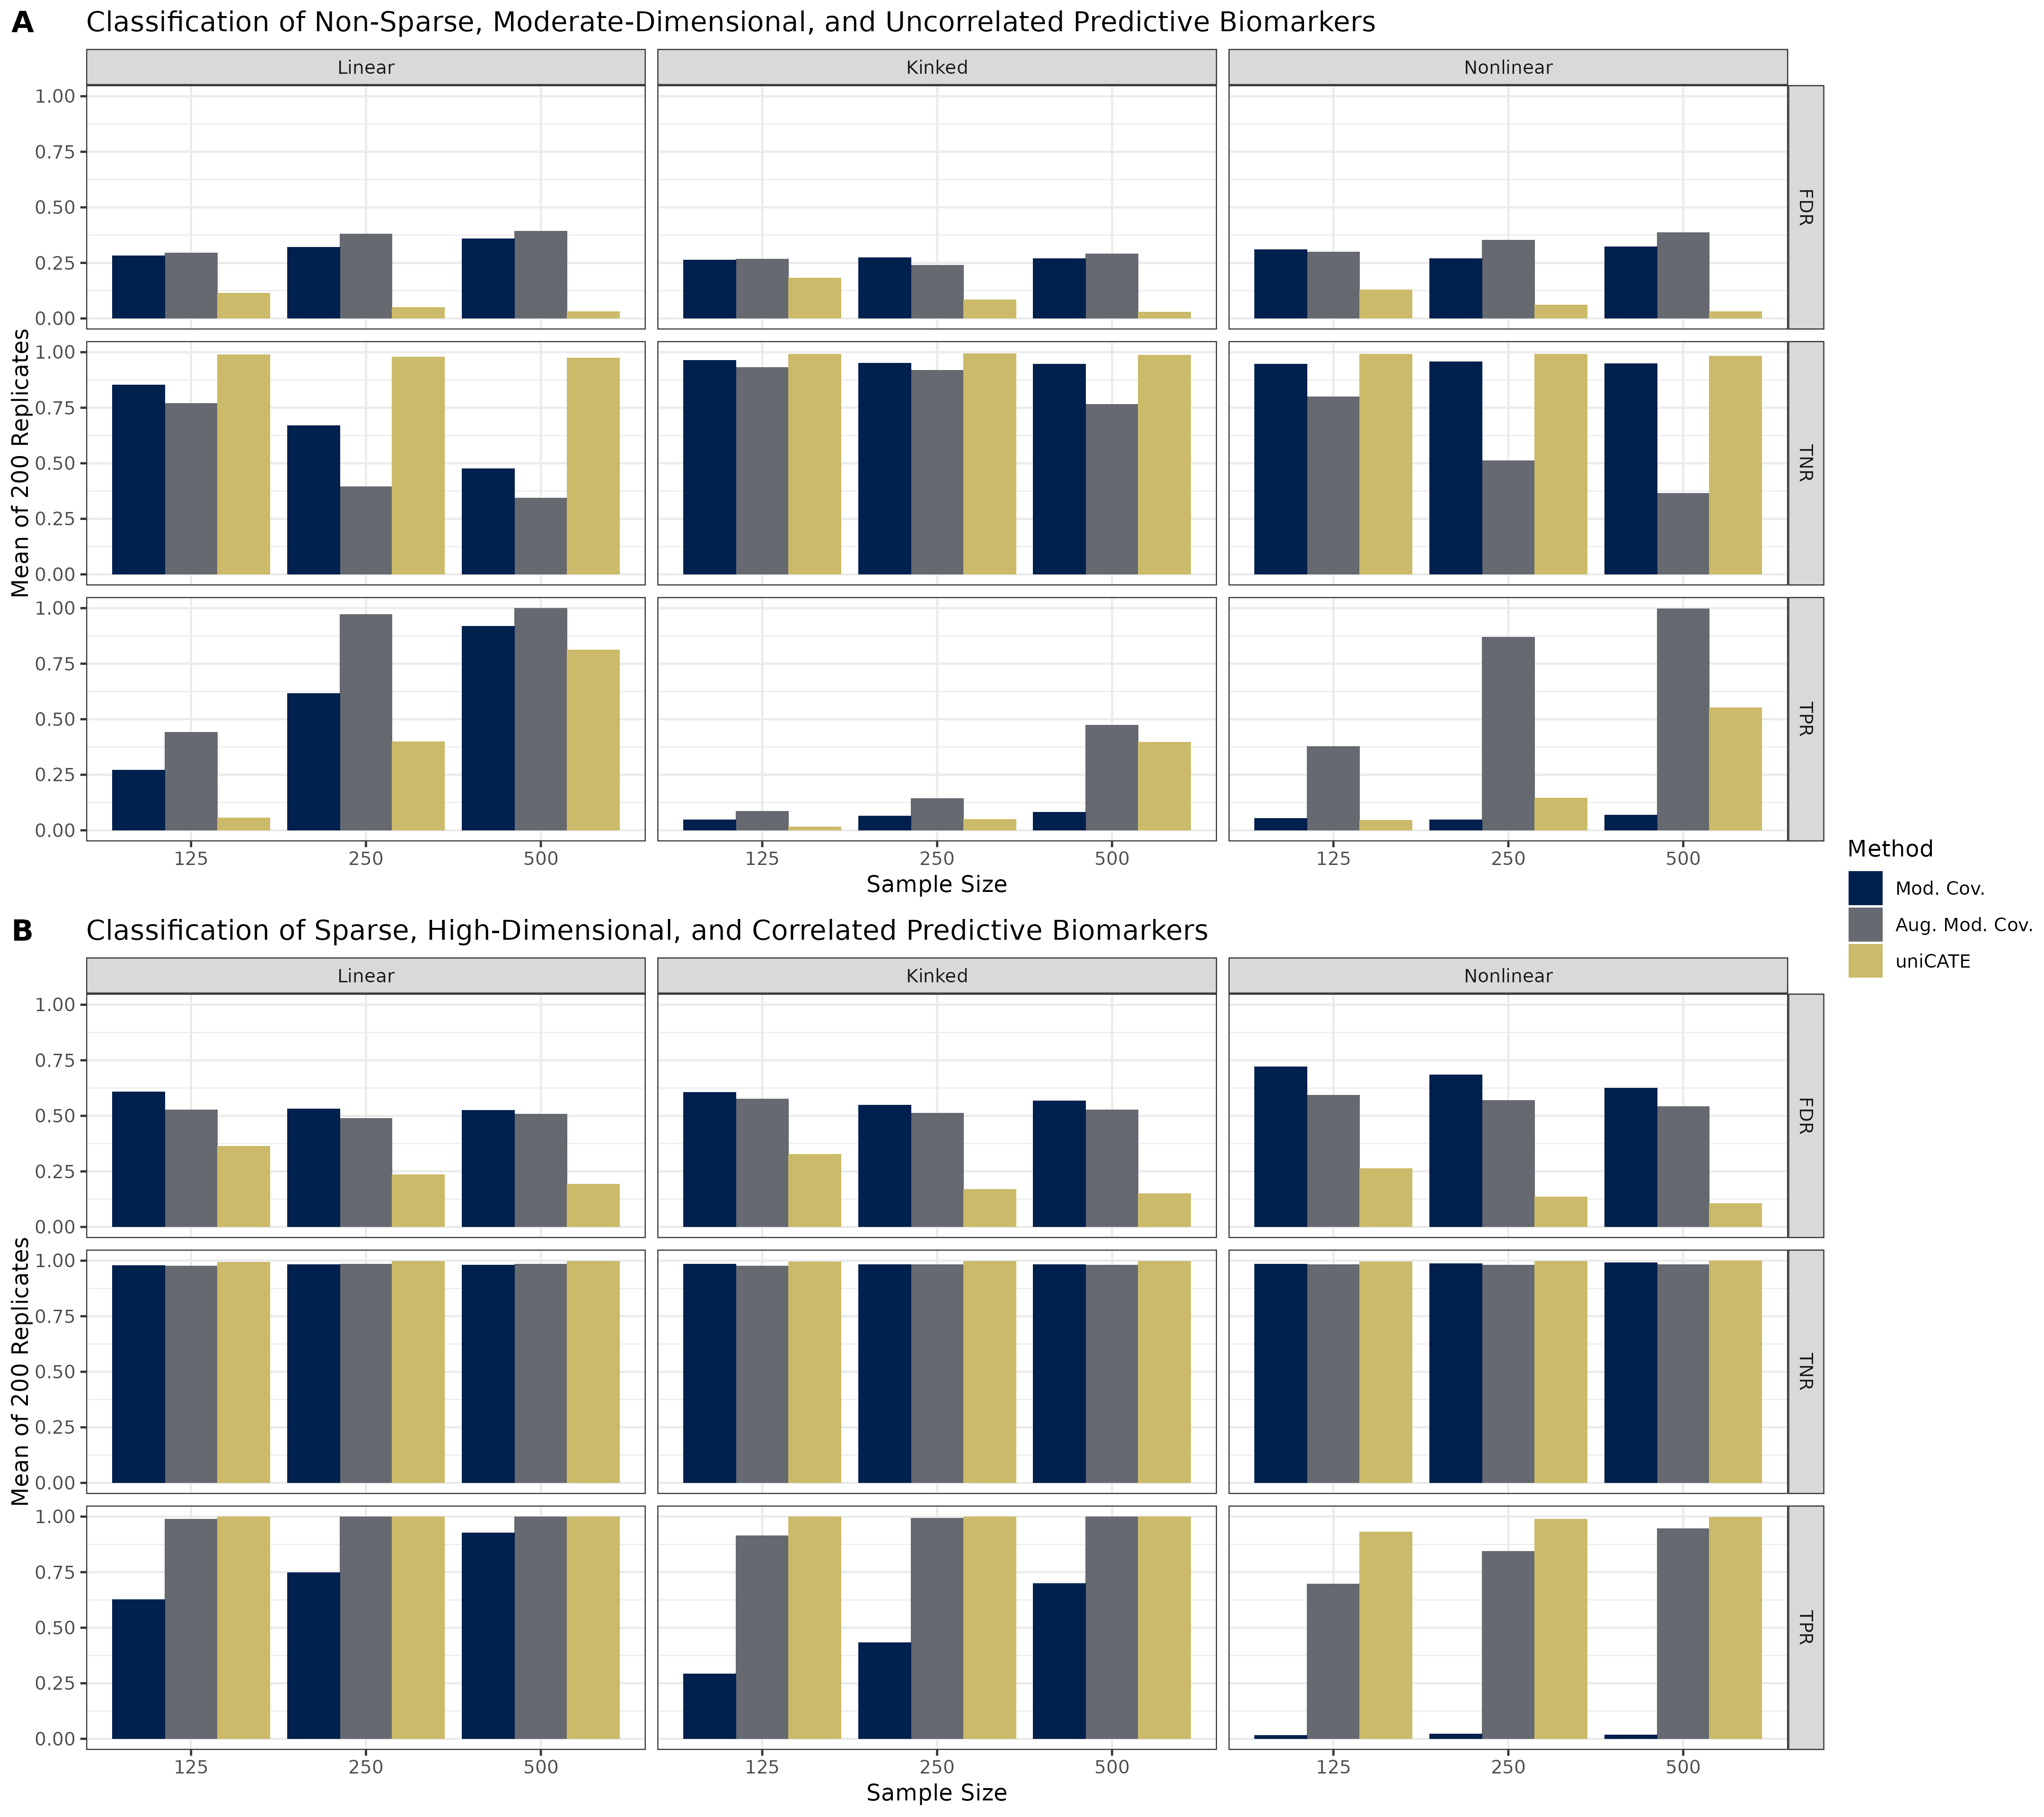
\includegraphics[width=0.29\textwidth]{graphs/classification-plot.png}
    \end{tikzfigure}
    \vspace{-2em}
  }

  \myblock{Conclusion}{
    Predictive biomarker discovery benefits from formal statistical inference
    procedures that control false discovery rates. This estimator is
    implemented in the \texttt{uniCATE} \texttt{R} package available at
    \texttt{github.com/insightsengineering/uniCATE}.
  }
  
  \mysmallblock{Reference}{
    \vspace{-1em}
    Tian et al. (2014) A Simple Method for Estimating Interactions
    Between a Treatment and a Large Number of Covariates, Journal of the
    American Statistical Association, 109:508, 1517-1532,
    DOI: 10.1080/01621459.2014.951443
    \vspace{-1em}
  }

\end{columns}

\end{document}
